\documentclass[11pt]{report}

\usepackage{
    courier,
    pdfpages,
    geometry,
    float
}

\title{Lab 4 Report}
\author{Connor Cimowsky\protect\\20427800}
\date{July 24, 2015}

\begin{document}

\maketitle

The scheduling diagram of my submission can be seen in Figure~\ref{fig:timing}.
In order to maximize processor utilization, it uses the earliest deadline first
(EDF) algorithm for scheduling tasks. This report discusses some of the
difficulties I encountered in the process of designing the scheduler.\\

\begin{figure}[h]
	\centering
	\makebox[\textwidth][c]{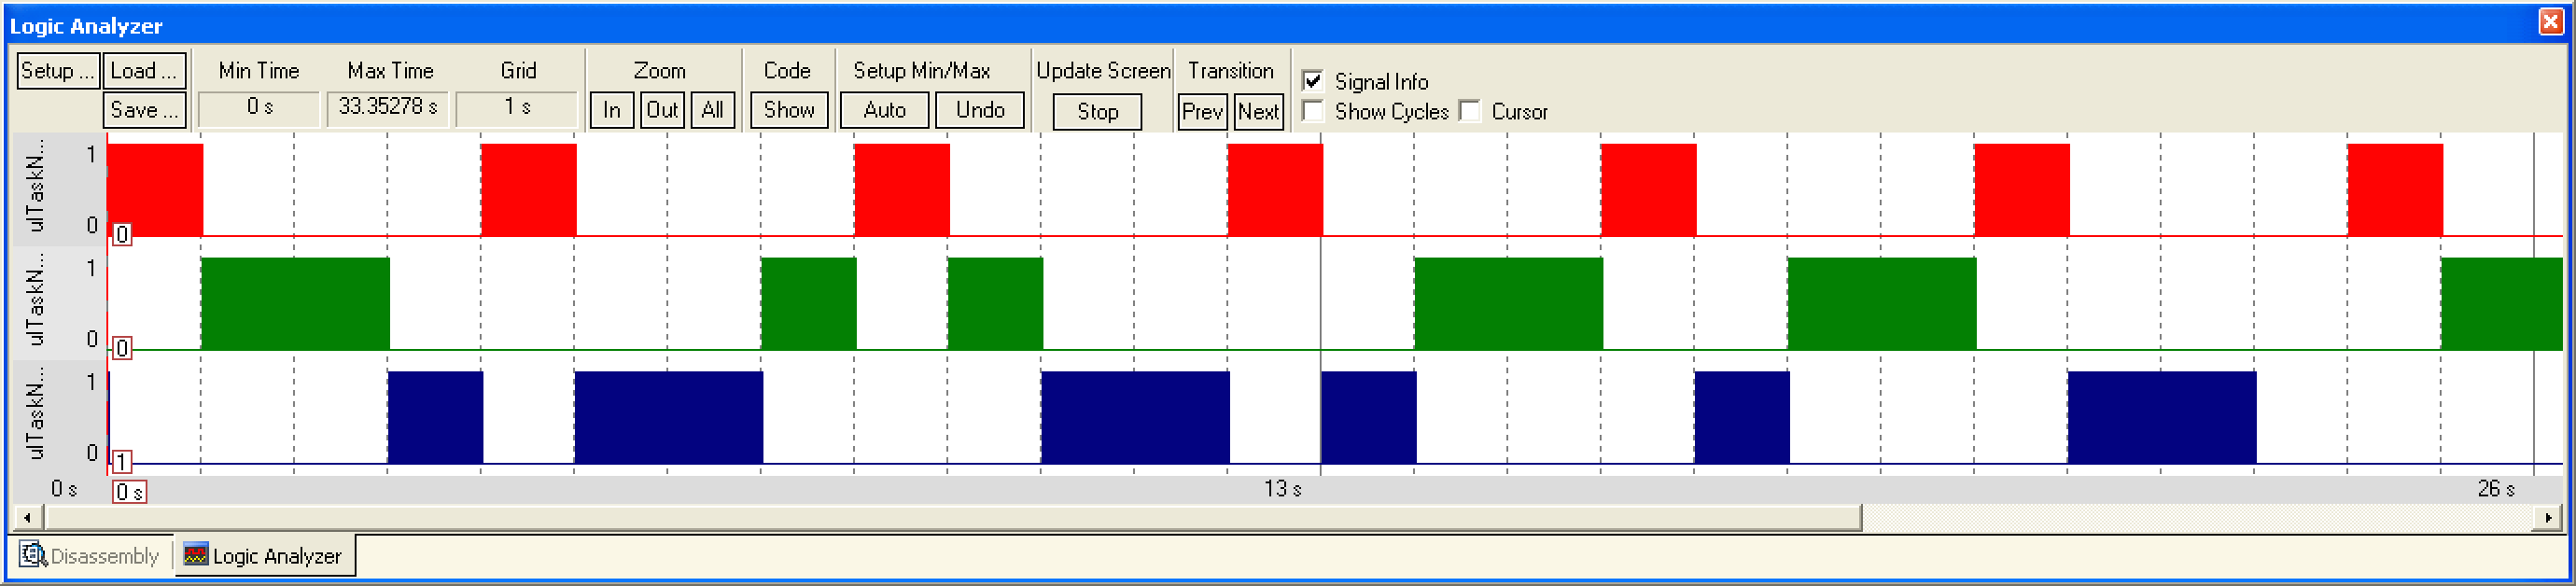
\includegraphics[width=1.2\textwidth]{timing}}
	\caption{Scheduling Diagram}
	\label{fig:timing}
\end{figure}

The first problem I encountered is that tasks would get scheduled too
frequently. For example, T1 would get scheduled at time 0, 2, and 4, even
though it should only be scheduled at time 0 and 4. After some debugging, I
realized that I needed a separate queue for tasks that have finished but have
not yet reached their deadline. This prevents them from being selected by the
EDF algorithm (which only looks at the ready queue). I also needed to add a
\texttt{wake\_time} field to the task control block (TCB) structure so that my
scheduler knows when to move tasks back into the ready queue. This also solved
another problem I had: even when no tasks should be scheduled (as is the case
at time 23), my scheduler would still select a task for execution; this was
because the tasks were still in the ready queue. When I added the separate
queue for blocked tasks, this problem went away.\\

Another problem I faced is that tasks would occasionally alternate for a few
time slots before eventually returning to normal. I realized that this was
because my scheduler did not break ties in the case when multiple ready tasks
had the same deadline. To fix this, I modified my EDF algorithm to prioritize
lower-numbered tasks when this scenario arises.\\

One final design decision that I had to make was whether to use priorities or
explicit task suspension for controlling task execution. Although the dynamic
assignment of priorities is easier to reason about, it introduces significant
complexity in the scheduler. This is because the actual scheduling of tasks is
then delegated to the FreeRTOS scheduler, making it difficult to know with
certainty which task will execute next. For this reason, I chose to explicitly
suspend and resume tasks from the scheduler (using the EDF algorithm for task
selection).

\end{document}
